Para trabajar con el problema de agrupamiento se utilizó el \textit{datset} ``Lung Cancer Prediction'', que puede consultarse en la página de Kaggle. Dicho \textit{dataset} tiene  mil registros de pacientes con cáncer de pulmón, cuenta con  25 características, entre las que se encuentran; edad, género, contaminación del aire, riesgo genético, dolor de pecho y el nivel de su condición (bajo, medio y alto). Si bien esta última característica podría permitirnos considerar a los datos como etiquetados, no la tomaremos en cuenta para poder trabajarlos con métodos de aprendizaje no supervisado. 

Las versiones de \textit{Python} y las librerías utilizadas fueron las siguientes:
\begin{itemize}
	\item  Pandas versión: 2.2.2
	
	\item  NumPy versión: 2.0.2
	
	\item  Seaborn versión: 0.13.2
	
	\item  Matplotlib versión: 3.10.0
	
	\item Sklearn versión: 1.6.1
	
	\item SciPy versión: 1.14.1
\end{itemize}

Como ya se mencionó, los registros tienen la característica \textit{'Level'}, por lo que el objetivo de esta sección es implementar métodos de agrupamiento para generar 3 \textit{clústeres} que nos permitan agrupar nuestros de manera similar a la característica \textit{'Level'}, debido a esto utilizaremos métodos de no jerárquicos, posteriormente utilizaremos el método \textit{PCA} para reducir la dimensión de nuestra \textit{dataset} para poder visualizar los \textit{clústeres} generados en gráficos 2D y 3D, finalmente compararemos los resultados que obtuvimos del agrupamiento con los datos originales para conocer la precisión que obtuvimos.

Primero hacemos una copia del \textit{dataset} con el que estamos trabajando y eliminamos las características \textit{'index', 'Patient ID'} y \textit{'Level'}, pues las primeras dos no son relevantes para el agrupamiento y ya planteamos que la última la usaremos para conocer la precisión que obtuvimos.

\subsubsection{Agrupamiento con k-means}

\lstset{
    language=Python,
    basicstyle=\ttfamily\footnotesize,
    keywordstyle=\color{blue},
    commentstyle=\color{gray},
    stringstyle=\color{green!60!black},
    numberstyle=\tiny\color{gray},
    numbers=left,
    breaklines=true,
    frame=single,
    captionpos=b,
    tabsize=4,
    showspaces=false,
    showstringspaces=false,
    showtabs=false
}
		
\begin{lstlisting}
    cancer_data = df.drop(columns=["Patient Id", "Level", "index"])

    # Estandarizamos los datos 
    scaler = StandardScaler()
    scaled_data = scaler.fit_transform(cancer_data)

    # Los convertimos en una data frame
    scaled_data_df = pd.DataFrame(scaled_data, columns=cancer_data.columns)
\end{lstlisting}

\begin{lstlisting}[caption={Código de k-means}]
    # posibles grupos: Low, Medium y High
    kmeans = KMeans(n_clusters=3, random_state=42, n_init=10)
    kmeans.fit(scaled_data)

    scaled_data_df['cluster'] = kmeans.labels_
\end{lstlisting}

Hacemos una reducción de dimensiones para poder visualizar los datos en 2D y 3D.  

\begin{lstlisting}[caption={PCA para 2D}]
    pca = PCA(n_components=2)
    cancer_pca = pca.fit_transform(scaled_data)
    print(f"Varianza total explicada: {sum(pca.explained_variance_ratio_)*100:.2f}%")
\end{lstlisting}

\begin{lstlisting}[caption={PCA para 3D}]
    pca3 = PCA(n_components=3)
    cancer_pca3 = pca.fit_transform(scaled_data)
    print(f"Varianza total explicada: {sum(pca3.explained_variance_ratio_)*100:.2f}%")
\end{lstlisting}

\begin{figure}[!ht]
    \centering
    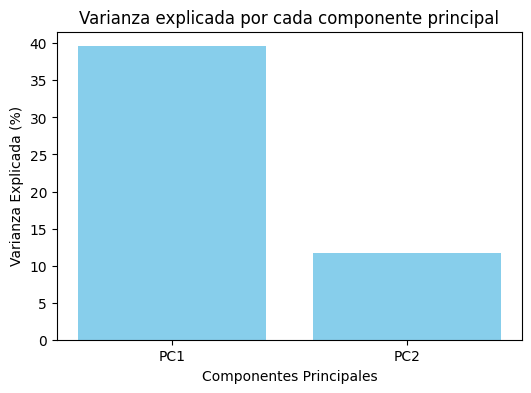
\includegraphics[scale = 0.75]{Enrique/Imagenes/Varianza_2d.png}
    \caption{Varianza de 51.32\%}
\end{figure}

\begin{figure}[!ht]
    \centering
    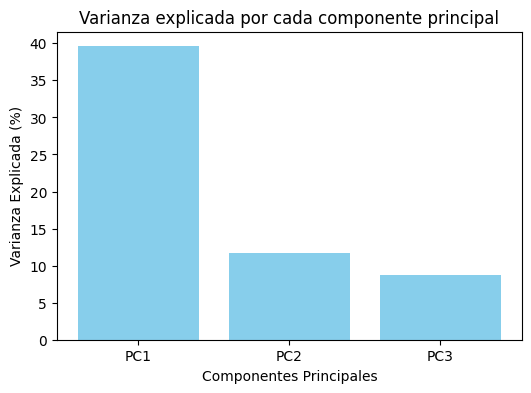
\includegraphics[scale = 0.75]{Enrique/Imagenes/varianza_3d.png}
    \caption{Varianza de 60.09\%}
\end{figure}

\subsubsection{Agrupamiento con DBSCAN}

También implementaremos el agrupamiento con el método \textit{DBSCAN}. Los primeros valores que proponemos para $\varepsilon$ y el número mínimo de muestras son 0.5 y 20 respectivamente, de lo cual obtenemos.

\begin{lstlisting}[caption={DSCAN con $\varepsilon$=0.5}]
    from sklearn.cluster import DBSCAN

    dbscan = DBSCAN(eps=.5, min_samples=20)
    dbscan.fit(scaled_data)

    print(dbscan.labels_.min(), dbscan.labels_.max())
\end{lstlisting}

\begin{lstlisting}[caption={Salida del código}]
    -1  9 
\end{lstlisting}

El -1 nos indica que el algoritmo clasificó algunos datos como \textit{atípicos}, que la etiqueta más grande sea 9 quiere decir que el algoritmo formó 10 grupos, como solo queremos formar 3 grupos, correremos el algoritmo para distintos valores de $\varepsilon$ hasta que solo se formen 3 \textit{clústeres}.

\begin{lstlisting}
    i = 0.5
    
    while dbscan.labels_.max() > 2:
        i += 0.1
        dbscan = DBSCAN(eps=i, min_samples=20)
        dbscan.fit(scaled_data)
        print(i, dbscan.labels_.min(), dbscan.labels_.max())
\end{lstlisting}

Con esto encontramos que la $\varepsilon$ que nos permite tener 3 grupos es 4.7, pero el algoritmo sigue clasificando algunos datos como atípicos, por lo que De manera similar encontramos el número de puntos mínimos

\begin{lstlisting}
    j = 20
    
    while dbscan.labels_.min() < 0 :
        j -= 1
        dbscan = DBSCAN(eps=4.9, min_samples=j)
        dbscan.fit(scaled_data)
        print(j, dbscan.labels_.min(), dbscan.labels_.max())
\end{lstlisting}

Finalmente obtenemos que $\varepsilon  =4.9$ y \textit{min\_samples = 19}, por lo que utilizaremos estos parámetros para el método \textit{DBSCAN}. Las etiquetas que obtengamos las guardaremos en una columna del \textit{dataframe scaled\_data\_df}

\begin{lstlisting}
    dbscan = DBSCAN(eps=4.9, min_samples=19)
    dbscan.fit(scaled_data)

    scaled_data_df['cluster DBSCAN'] = dbscan.labels_
\end{lstlisting}